\chapter{Podstawy teoretyczne i omówienie koncepcji proponowanego rozwiązania}
  
  W poprzednim rozdziale opisano przykładowe narzędzia funkcjonujące na rynku oprogramowania do zarządzania wymaganiami. Opisano ich główne wady i zalety oraz przedstawiono najważniejsze problemy związane ze stosowaniem ich w praktyce.

  W tym rozdziale, zostaną opisane procesy inżynierii wymagań od strony teoretycznej. Zostanie również zwrócona uwaga na niezbędne elementy nowoczesnego systemu wspierającego pracę z wymaganiami w małych i średnich przedsiębiorstwach. Na koniec rozdziału, przedstawiona zostanie koncepcja nowego narzędzia, będącego przedmiotem tej pracy.
  
  \section{Inżynieria wymagań}
    
    Inżynieria wymagań (IW) jest dziedziną, na którą składają się wszelkie działania związane z odkrywaniem (elicitation), analizą (analysis), weryfikacją (validation) oraz zarządzaniem wymaganiami \cite{Somm06}. Dotyczy ona każdego systemu informatycznego, niezależnie od jego rozmiarów i jest jednocześnie jednym z najistotniejszych procesów w cyklu życia projektu.

    IW dostarcza metodologii i narzędzi, służących do precyzyjnego określenia celu i zakresu projektu, poprzez identyfikację interesariuszy i ich potrzeb oraz udokumentowanie wyników w formie umożliwiającej ich analizę, komunikację oraz finalnie - implementację \cite{Nus00}. 

      \subsubsection{Zarys historyczny}

        Kryzys oprogramowania na przełomie lat '60 i '70 XX wieku był katalizatorem do podjęcia prób usystematyzowania młodej wówczas dziedziny tworzenia systemów informatycznych. Był to okres popularyzjacji sprzętu komputerowego, powszechnego, dramatycznie rosnącego zapotrzebowania na programistów oraz nagłośnionych, wielkich porażek systemów informatycznych, jak katastrofa rakiety kosmicznej Mariner 1 \cite{Brooks75}. Niedobór wykwalifikowanych programistów, zmusił korporacje do intensywnych poszukiwań nowych rozwiązań. Literatura branżowa szybko przepełniła się głosami nawołującymi do poprawy metod zarządzania w projektach informatycznych. Pojawiły się takie tytuły jak ‘‘Controlling Computer Programming’’, ; ‘‘New Power for Management’‘; ‘Managing the Programming Effort’’; ‘‘The Management of Computer Programming Efforts’’. W roku 1968, w drodze ustaleń na konferencji NATO Software Engineering (tu po raz pierwszy w branży zaczęto mówić o ,,kryzysie oprogramowania''), ''zarządzanie oprogramowaniem'' stało się fundamentem i jednym z głównych dyskursów w dziedzinie inżynierii oprogramowania \cite{Ense03}.
        
        Pionierzy inżynierii oprogramowania podejmowali próby zaczerpnięcia wiedzy z zakresu inżynierii systemów i wykorzystania jej w projektach informatycznych. Ten kierunek rozwoju opierał się na paradygmacie klasycznej inżynierii, zakładającym budowę systemu zgodną z określonym procesem: od identyfikacji problemu, opracowaniu specyfikacji, konstrukcji systemu i jego utrzymania. Takie sekwencyjne podejście do tworzenia systemów informatycznych było fundamentem powstania pierwszych procesów wytwórczych oprogramowania. 
        
        Klasycznym podejściem był przedstawiony w pracy Winstona Royce'a (1970), model kaskadowy (sekwencyjny model liniowy)\footnotemark. \footnotetext{Royce podał w swoim modelu wariant liniowego procesu, gdzie kolejne fazy były zwrotnie sprzężone z fazami poprzednimi \cite{RWins70}, jednak w większości organizacji stosujących model kaskadowy, jest to ściśle sekwencyjny proces liniowy \cite{pressman2010software}.} W swojej pracy, Royce proponując rozwiązanie sekwencyjne (w którym żaden kolejny etap nie mógł zostać rozpoczęty przed zakończeniem etapu poprzedniego) zastrzegł, że ,,wierzy w zaproponowaną koncepcję, jednak jej implementacja jest ryzykowna i naraża projekty na niepowodzenie'' \cite{RWins70}. Zatem już na samym początku swojego istnienia, model kaskadowy wraz z analogią inżynierii oprogramowania do inżynierii klasycznej, był uważany w branży za nieprzystosowany do dziedziny problemu. Mimo tego, model kaskadowy, z powodzeniem, znalazł zastosowanie w dużych projektach m. in. rządowych, wojskowych i kosmicznych, gdzie zarówno klient jak i wykonawcy bardzo dobrze rozumieli wymagania systemu \cite{NasaSE}. W kolejnych latach pojawiały się modyfikacje modelu kaskadowego, a rola podejścia iteracyjnego przybierała na znaczeniu. W roku 1986 Barry Boehm opisał model spiralny, będący połączeniem ustrukturalizowanego procesu kaskadowego z rozwojem przyrostowym, opartym na prototypowaniu \cite{Boehm86}. Kolejnym kamieniem milowym w dziedzinie procesów wytwórczych oprogramowania było wydanie książki Kent'a Beck'a ,,Extreme Programming Explained'' \cite{KBeck00} w roku 1999 oraz publikacja ,,Agile Manifesto'' w roku 2001, gdzie po raz pierwszy, formalnie zaproponowano termin ,,zwinnego programowania'' \cite{MFowl01}. 
      
      \subsubsection{Podobieństwa w procesach wytwórczych}

        Pomimo znaczących różnic w dostępnych i udokumentowanych metodykach projektowych, dla wszystkich istnieje część wspólna, w postaci nieuniknionej fazy analizy na etapie rozpoczęcia projektu. Nie ma możliwości rozpoczęcia modelowania ani implementacji systemu, bez wcześniejszej wiedzy w zakresie jego przeznaczenia i oczekiwanych funkcji. Zarówno w metodykach zwinnych, jak i w tradycyjnych procesach wytwórczych, w początkowej fazie projektu, kluczową rolę gra przygotowanie systemu od strony wymagań. Zatem inżynieria wymagań dotyczy każdego procesu wytwórczego.

      \subsubsection{Procesy w inżynierii wymagań}

      Jak podaje Sommerville \cite{Somm06}, do dziedziny inżynierii wymagań możemy zaliczyć następujące pod-procesy:

      \begin{itemize} 
          \item studium wykonalności 
          \item gromadzenie i analiza wymagań
          \item weryfikacja wymagań
          \item zarządzanie wymaganiami
      \end{itemize}

      \subsubsection{Studium wykonalności (feasibility study)}

        Wg. Sommerville'a (2006), przy dużych projektach, w początkowym stadium powinno zostać przeprowadzone studium wykonalności. Podstawowym celem jego przeprowadzania jest udzielenie odpowiedzi na pytanie, czy należy kontynuować projekt. W trakcie tego etapu zwiększa się wiedza o dziedzinie problemu, a koncepcja systemu jest weryfikowana pod kątem celowości zastosowania w organizacji, wszelkich ograniczeń systemowych, a także sprzętowych. W modelu Rational Unified Process, studium wykonalności powinno zostać włączone do fazy rozpoczęcia projektu (inception phase) \cite{Kruch03}.

        W niektórych przypadkach (szczególnie w dużych projektach krytycznych) studium wykonalności może zostać rozbudowane do pełnej analizy oceny ryzyka. Wówczas powinny zostać uwzględnione aspekty nietechniczne i administracyjne, np.: czy projekt ma przydzielony wystarczający budżet, jakie aspekty polityczne należy wziąć pod uwagę w trakcie definiowania wymagań, czy projekt może być wykonany w przyjętych ramach czasowych.

      \subsubsection{Gromadzenie i analiza wymagań}

        Gromadzenie wymagań jest procesem, na który składają się działania zmierzające do zgłębienia celu i motywacji przyświecających budowie analizowanego systemu. W szczególności etap ten wiąże się z identyfikacją wszystkich wymagań, jakie musi spełnić system, aby osiągnąć sukces.
        
        Proces gromadzenia wymagań w języku angielskim nosi nazwę ,,requirements elicitaion''. ,,Elicitaion'' w dosłownym tlumaczeniu, oznacza ,,wywołanie'', ,,wydobycie'', ,,ujawnienie''. W szczególności termin ,,wydobycie'' lepiej oddaje naturę tych działań, niż popularne w języku polskim ,,gromadzenie'' czy ,,definiowanie'' wymagań. Innymi słowy jest to proces komunikacji analityków z użytkownikami w celu zdobycia jak największej ilości informacji o budowanym systemie. 

        Głównymi technikami związanymi z pozyskiwaniem wymagań są: identyfikacja interesariuszy, gromadzenie faktów i informacji przy pomocy wywiadów, kwestionariuszy, list kontrolnych, warsztatów kreatywnych, burzy mózgów, map myśli (mindmapping), modelowania i prototypowania. Znaczna część wymagań stanowi wiedzę zdobytą w procesie przeprowadzania wywiadów z interesariuszami projektu. W związku w powyższym, można wprowadzić uniwersalne uogólnienie, stwierdzając, że głównym narzędziem wykorzystywanym w procesie gromadzenia wymagań jest szeroko rozumiana komunikacja. Wywiady przeprowadzane z interesariuszami mogą mieć formalny lub nieformalny przebieg, a stosowane w tym procesie narzędzia w dużej mierze zależą od poziomu skomplikowania projektu, wypracowanych metod, dostępnych narzędzi i preferencji samych analityków. 
        
        Wymagania zwykle pochodzą z wielu heterogenicznych źródeł. Najwyższy priorytet zawsze powinien przysługiwać wymaganiom pochodzącym od klienta i użytkowników systemu. Jednak wpływ na specyfikację systemu mogą mieć również źródła zewnętrzne, takie jak niezależni eksperci z dziedzin obejmowanych przez projekt, uwarunkowania prawne i ekonomiczne, czy ogólnie przyjęte standardy i procedury związane ze szczególnymi aspektami tworzonego systemu.

        Dokumentem stanowiącym rezultat pracy nad gromadzeniem wymagań jest specyfikacja wymagań systemu. Standardem określającym proces tworzenia i strukturę tego dokumentu jest IEEE Guide for Developing System Requirements Specifications \cite{institute1984ieee}. Wiele organizacji definiuje również własne standardy i procesy, lepiej odpowiadające specyfice realizowanych projektów.

        Do procesu gromadzenia wymagań i narzędzi z nim związanych, autor powróci przy okazji opisu koncepcji proponowanego rozwiązania, w następnym rozdziale.

      \subsubsection{Weryfikacja wymagań}

        Celem procesu weryfikacji wymagań jest dowiedzenie, że koncepcja budowanego systemu odpowiada rzeczywistym potrzebom użytkowników. Jest to kluczowy proces inżynierii wymagań, ponieważ poprawa zidentyfikowanych na tym etapie problemów jest o rząd wielkości mniej kosztowna, niż późniejsze zmiany systemowe. Zdecydowanie łatwiej jest bowiem poprawiać projekt architektury opgrogramowania niż wprowadzać modyfikacje koncepcyjne w istniejącym już systemie. 

        Weryfikacja wymagań powinna być przeprowadzana na podstawie dokumentu specyfikacji wymagań systemu. Działania podejmowane w trakcie weryfikacji wymagań powinny uwzględniać przede wszystkim zasadność, bezkonfliktowość, kompletność, implementowalność i weryfikowalność wszystkich wymagań. Zasadność pozwala odpowiedzieć na pytanie, czy dane wymaganie rozwiązuje realny problem w systemie, potwierdzając tym samym celowość swojego istnienia. Ponieważ w trakcie gromadzenia wymagań przeprowadzane są wywiady z wieloma interesariuszami projektu, mającymi różne, często sprzeczne wymagania, konieczna jest weryfikacja spójności specyfikacji pod względem konfliktów. Zapewnienie bezkonfliktowości polega na takim sfomułowaniu wymagań w specyfikacji, aby żadne nie były ze sobą w sprzeczności. Kompletność jest weryfikacją dokumentu wymagań z perspektywy realizacji wszystkich porządanych funkcji. Wszystkie zdefiniowane wymagania muszą być realizowalne w określonym czasie, przy użyciu określonego sprzętu i opgrogramowania. W trakcie badania implementowalności, analityk skupia się na odpowiedzi na pytanie czy dane wymaganie jest w pełni realizowalne w rzeczywistych warunkach. Z kolei weryfikowalność ma na celu zapewnienie narzędzi, umożliwiających sprawdzenie i demonstrację poprawności działania zrealizowanego wymagania za pomocą metod empirycznych.

        Istnieje wiele narzędzi i metod, jakie można wykorzystać w procesie weryfikacji wymagań. Wyniki badania Boehem et al ,,Prototyping vs. Specifying'' \cite{Boehm84} dowodzą, że jedną ze skuteczniejszych metod prewencji przed definiowaniem błędnych wymagań jest metoda prototypowania. Badanie to polegało na podziale grupy studentów inżynierii oprogramowania na dwa zespoły. Celem obu zespołów była implementacja systemu o określonym zakresie. Jedna grupa korzystała z metody prototypowania. Ich konkurenci, natomiast, korzystali z podejścia zorientowanego na specyfikację. W rezultacie, grupa stosująca metodę prototypowania osiągnęła lepsze wyniki, w szczególności, w zakresie użyteczności interfejsu użytkownika i prostoty obsługi dostarczonego systemu. W przeciwieństwie do podejścia opartego na samej specyfikacji, prototypowanie umożliwia wizualizację wymagań systemu, uniezależniając interpretację treści wymagania od wyobraźni odbiorcy. 

        Jednak, jak każda metoda, prototypowanie nie jest wolne od wad. Istnieje ryzyko, że prototyp, kładąc zbyt duży nacisk na pewne szczegóły, sprawi, że ogólna koncepcja systemu przestanie być wyraźnie dostrzegalna. Ponadto, wyzwaniem w przypadku prototypowania jest odpowiednia komunikacja z klientem. Klient musi dokładnie rozumieć specyfikę i cel tworzenia prototypu. Istnieje bowiem pokusa, aby pod naciskami klienta wykorzystać prototyp jako finalny produkt. W związku z powyższym, wśród wszystkich członków zespołu, niezbędna jest pełna świadomość faktu, iż prototyp, po spełnieniu swojej funkcji zostanie odstawiony, a doświadczenia z jego budowy posłużą jako informacje wejściowe do implementacji finalnego rozwiązania. Powstało wiele prac dotyczących prototypowania, jednak szczegółowe aspekty tego podejścia wykraczają poza zakres tej pracy. Osoby zainteresowane metodami prototypowania znajdą kilka ciekawych pozycji w bibliografii \cite{arnowitz2006effective, budde1992prototyping}.

      \subsubsection{Zarządzanie wymaganiami}

        Specyfika większości projektów informatycznych, wiąże się z tym, że raz udokumentowane wymagania rzadko pozostają aktualne do momentu zakończenia prac. Wymagania są przedmiotem ciągłych zmian i niezbędne są narzędzia, których zadaniem będzie zarządzanie tymi zmianami. Proces zarządzania wymaganiami należy rozpocząć w momencie powstania pierwszej wersji specyfikacji wymagań i kontynuować aż do zakończenia projektu.

  \section{Język UML w trakcie fazy analizy}
    ** opis teoretycznych aspetków zastosowania języka UML w trakcie fazy analizy ze szczególnym uwzględnieniem etapu zebirania wymagań.    


  \section{Technologie webowe w kontekście RIA (zalety i wady przenoszenia sie do webu)}
    ** Rich Internet Applications i możliwości jakie niesie ze sobą ten kierunek rozwoju w kontekście inżynierii wymagań **


  \section{Motywacja podjęcia prac nad nowym rozwiązaniem}

    Mając na uwadze teoretyczne tło dziedziny jaką jest inżynieria wymagań oraz praktyczne problemy z jakimi borykają się dzisiaj małe i średnie przedsiębiorstwa w zakresie zarządzania wymaganiami, powstała koncepcja rozwiązania, adresującego najpilniejsze problemy w rzeczywistych projektach małej i średniej skali. 

    Jak wykazano w rozdziale 2, pomimo rozwoju technologii oraz świadomości firm w zakresie inżynierii oprogramowania, bardzo duża część małych \linebreak i średnich przedsiębiorstw nadal ignoruje zagadnienia z zakresu inżynierii wymagań. Dojrzałość tych organizacji pod kątem inżynierii oprogramowania jest bardzo niska. Niewielką część harmonogramów projektów przeznacza się na analizę wymagań, a narzędzia stosowane w trakcie tego procesu najczęściej ograniczają się do pakietów biurowych, klientów poczty elektronicznej i odręcznych notatek. Mikro-firmy osiągająjące na tym polu sukcesy najczęściej charakteryzują się posiadaniem bardzo małych zespołów ekspertów z ogromym doświadczeniem w branży, posiadającymi techniki wypracowane metodami prób i błędów, nad którymi pracowali przez wiele lat w swojej karierze.  Jednak zdecydowana większość firm nadal eksperymentuje z autorskimi podejściami, często integrując różne istniejące narzędzia. 
    
    Część winy za taki stan rzeczy leży po stronie twórców oprogramowania. Istnieje niewiele systemów umożliwiających skuteczne zarządzanie wymaganiami w środowsiku dynamicznych, zorientowanych na rynek internetowy, projektów, jakie najczęściej realizują firmy z sektora MŚP. Kolejną ważną obserwacją jest fakt, iż bardzo często mamy do czynienia z projektami, których wymagania wymyślane są przez samych twórców, przez co proces dokumentowania wymagań i tworzenia specyfikacji przebiega ad hoc lub nie istnieje w ogóle. Dodatkowo, brak umiejętności zarządzania zmianą, powoduje, że projekty oddawane są po terminie, z przekroczonym budżetem, często niedostarczając klientowi porządanego efektu. Jest to problem całej branży - zarówno kadry zarządzającej, analityków, programistów, klientów i użytkowników. Problemy z zarządzaniem wymaganiami, powodują, spowolnienie innowacji. Gdyby firmy zaczęły umiejętnie zarządzać wymaganiami i zmianą, więcej projektów kończyłoby się sukcesem, co pozytywnie wpłynęłoby na prędkość rozwoju oprogramowania. Ewidentnie istnieje niezagospodarowana luka na rynku w tym segmencie. 

    Małe i średnie przedsiębiorstwa są motorem napędowym dzisiejszej gospodarki opartej w znacznym stopniu o techniki informacyjne. Obowiązkiem inżynierii oprogramowania jest stałe kwestionowanie istniejących rozwiązań i katalizowanie zmian w kierunku usprawniania procesów związanych z wytwarzaniem oprogramowania. Jednak inżynieria wymagań zdaje się być niedocenianym i nadal słabo rozumianym zagadanieniem związanym z wytwarzaniem oprogramowania. Jest to jednak kluczowa, przyszłościowa dziedzina - w miarę postępu technologicznego, zapotrzebowanie na oprogramowanie nadal będzie wzrastało.

  \section{Opis proponowanego rozwiązania}

    Proces pozyskiwania i przetwarzania wymagań powinien być przede wszystkim łatwy w implementacji dla organizacji oraz dający dużą dozę elastyczności. W rozdziale 'Problemy z istniejącymi rozwiązaniami' opisano stan sztuki i zaadresowano niedociągnięcia dzisiejszych narzędzi. 

    Motywem przewodnim proponowanego narzędzia jest przystępność i prostota obsługi oraz wniesienie rzeczywistej wartości dodanej poprzez dostarczenie funkcji, mających realne zastosowanie w praktyce. 

    W trakcie prac nad koncepcją narzędzia postawiono następujące cele:
    
    \begin{itemize}
      \item Ogólny przegląd stanu projektu - najistotniejsze informacje z perspektywy wymagań systemu powinny być dostępne na jednej stronie podsumowującej projekt
      \item Wsparcie gromadzenia wymagań - wsparcie pozyskiwania, definiowania, katalogowania (grupowania) nieprzetworzonych wymagań oraz nadawania im odpowiednich priorytetów
      \item Uniwersalność formatu przechowywanych danych - ułatwienie dalszego przetwarzania treści wymagań przez zewnętrzne systemy
      \item Dostarczenie rozwiązań zarządzania zmianą - wsparcie zarządzania wymaganiami na późniejszych etapach projektu
      \item Stworzenie centralnego repozytorium wiedzy na temat wymagań
      \item Wsparcie kolaboracji - umożliwienie współpracy wszystkich członków zespołu
      \item Automatyzacja tworzenia specyfikacji - implementacja algorytmu generującego dokument specyfikacji wymagań 
      \item Silna koncentracja na praktycznym zastosowaniu systemu wsparcia zarządzania wymaganiami(!) 
    \end{itemize}

    W efekcie powstał prototyp systemu, otwierający drogę do dyskusji i rozwoju w kierunku poprawienia procesów inżynierii wymagań w małych i średnich przedsiębiorstwach. 

  \section{System Reqmanager - opis funkcjonalności}

    \subsection{Ogólny przegląd stanu projektu}
      Ekranem głównym jest przegląd stanu projektu z perspektywy wymagań. Użytkownik ma możliwość natychmiastowej edycji głównej notatki opsiującej główne założenia całego projektu oraz jego krótki opis. Ponadto, dostępna jest lista wymagań zawierająca podstawowe informacje takie jak kod wymagania, jego opis, priorytet oraz ilość przypisanych przypadków użycia. Wszystkie te elementy umieszczone na jednej stronie, umożliwiają użytkownikowi ogólną orientację w zakresie i celach projektu pod kątem wymagań. 

    \subsection{Wsparcie gromadzenia wymagań}
      Praktyczne narzędzie do zastosowania w procesie gromadzenia wymagań musi wspierać najwcześniejszą fazę - powstawania wymagań. W dynamicznych projektach, wymagania pojawiają się niespodziewanie, w różych sytuacjach i pochodzą z wielu różnych źródeł. Narzędzie musi wspierać prostą w obsłudze opcję dodawania wymagań w postaci krótkich notek, dłuższych artykułów lub opisów całych procesów. Jednocześnie nie może obarczać użytkownika obowiązkiem nadawania identyfikatorów oraz innych meta-informacji. Powinno również ograniczać potrzebę formatowania treści. Celem użytkownika, jest spisanie jak najszybciej wszystkich obserwacji i zachowanie ich w formie możliwej do późniejszego przetworzenia.

      Proponowane rozwiązanie wspiera ten proces dzięki zintegrowanemu edytorowi tekstu, edytorowi diagramów przypadków użycia oraz systemowi załączników.
      
      Formatowanie tekstu w języku znaczników Markdown \cite{Grub04} umożliwia nadanie dokumentowi logicznej struktury wykorzystując zwykły tekst (plain text) zaopatrzony w odpowiednie oznaczenia. Dzięki temu użytkownik otrzymuje czytelny dokument, przy jednoczesnym ograniczeniu formy graficznej, która jest w tym konekście drugoplanowa.

      Edytor diagramów przypadków użycia umożliwia wzbogacenie treści wymagania o jego graficzną reprezentację. Moduł edycji diagramów przypadków użycia wspiera współdzielenie diagramów pomiędzy wieloma wymaganiami, umożliwiając oznaczanie odpowiednich elementów graficznych jako odpowiedzialnych za realizację aktualnie opracowywanego wymagania.

      System załączników dodatkowo wzbogaca możliwości ekspresji - do wymagania użytkownik może dodać dokumenty lub treści multimedialne powiązane z danym wymaganiem, mające na clu lepsze zrozumienie istoty problemu.

      \begin{figure*}[t]
        \centering
        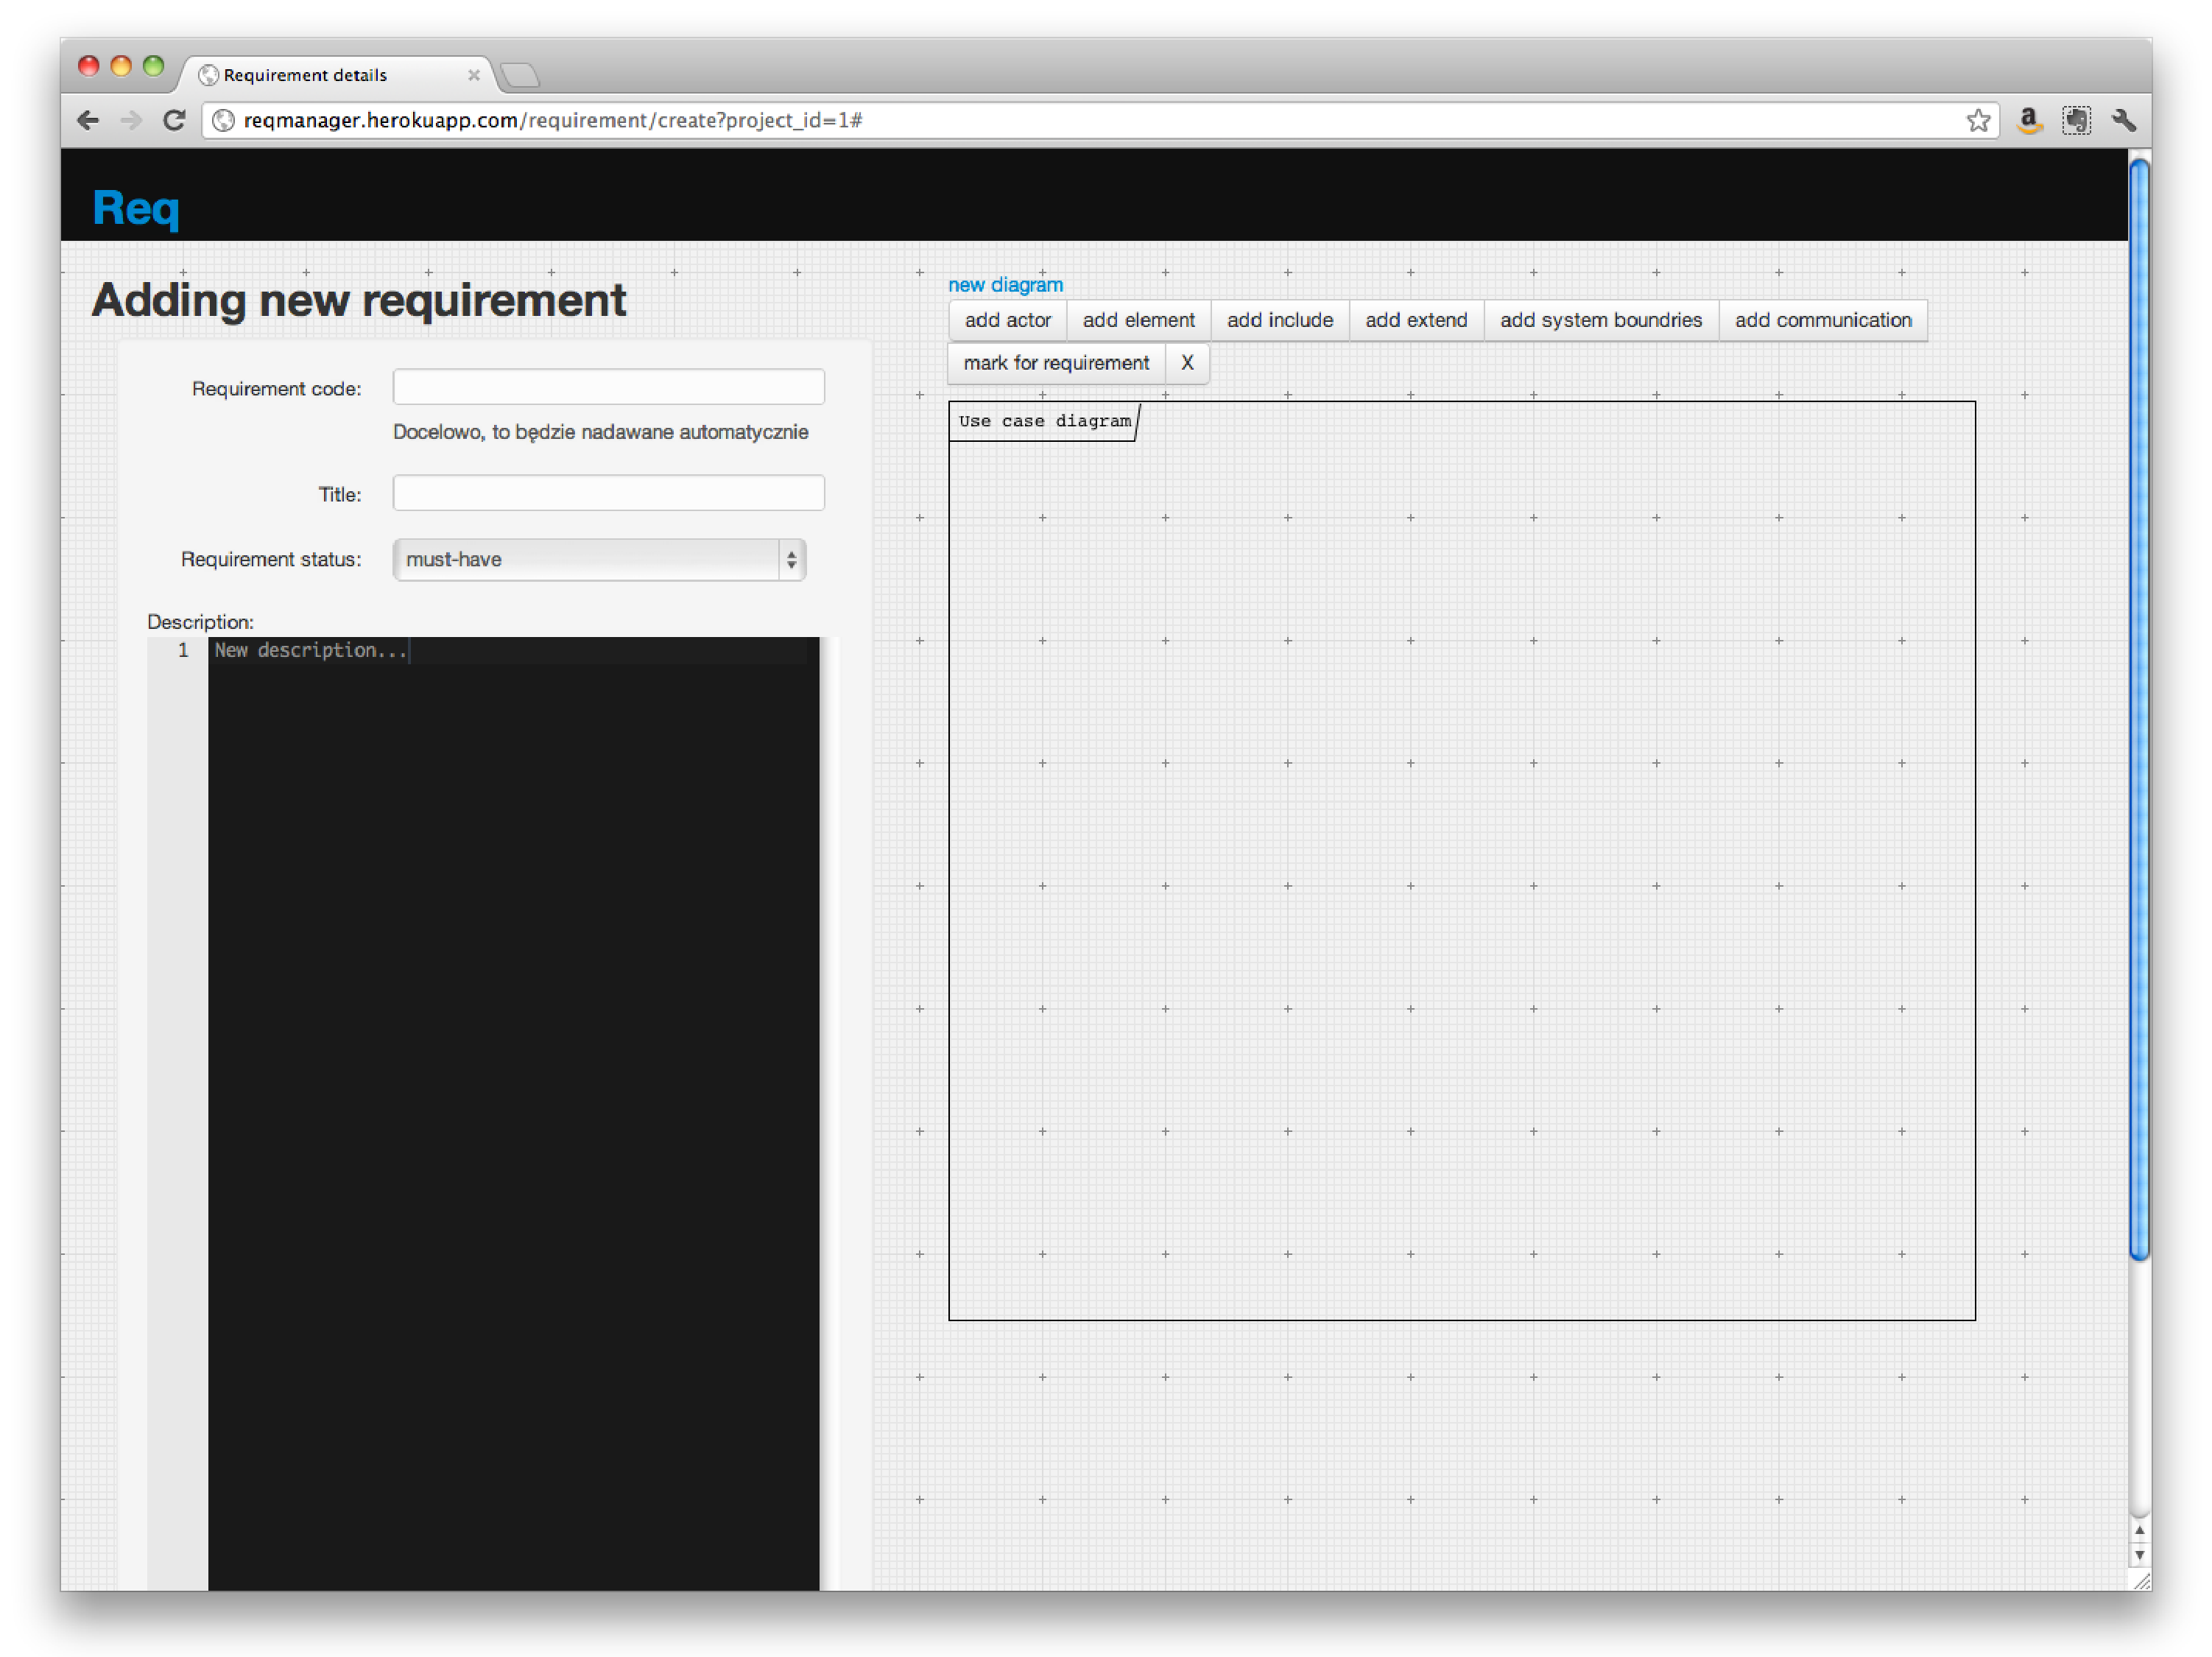
\includegraphics[width=1.0\textwidth]{screen_test.pdf}
        \caption{Test}
      \end{figure*}

    \subsection{Uniwersalność formatu danych}
      Dojrzałe narzędzie zarządzania wymaganiami powinno ułatwiać późniejsze procesowanie wprowadzonych do niego danych. Proponowany system realizuję tę potrzebę przechowując wszystkie wymagania oraz powiązane diagramy w bazie danych. Treść opisu wymagań jest przechowywana w postaci zwykłego tekstu, zaopatrzonego w znaczniki Markdown. Dzięki temu, treść wymagań jest znacznie łatwiejsza w przetwarzaniu, niż dokumenty tworzone przez klasyczne edytory tekstu.
      
      Ponadto, struktura diagramów powiązanych z wymaganiami jest przechowywana w bazie danych w formacie xml. Takie podejście również w zancznym stopniu ułatwia późniejsze przetwarzanie informacji zawartych na diagramach. 
      
      System aktywnie wykorzystuje powyższe właściwości podczas automatycznego generowania specyfikacji wymagań.

    \subsection{Zarządzanie zmianą}
      Zarządzanie zmianą jest istotne z punktu widzenia ewolucji wymagań i stopniowego uszczegóławiania dokumentacji systemu. Proponowane narzędzie wspiera ten proces zachowując poprzedni stan wymagania w trakcie jego zapisu. Dzięki temu możliwe jest prześledzenie zmian dokonywanych w wymaganiach. 

    \subsection{Centralne repozytorium}
      Proponowany system jest dostępny przez przeglądarkę, dzięki czemu stanowi centralne repozytorium wiedzy na temat wymagań w projekcie. Interfejs www z elementami html5 powoduje, że narzędzie wymaga jedynie nowoczesnej przeglądarki internetowej, bez żadnych dodatkowych wtyczek. Dzięki temu aplikacja cechuje się wysokim poziomem dostępności.  

    \subsection{Kolaboracja}
      Możliwość komentowania wymagań została zaimplementowana z myślą o umożliwieniu kolaboracji nad wymaganiami członkom zespołu.

    \subsection{Generator specyfikacji}
      Jedną z kluczowych funkcjonalności proponowanego rozwiązania jest automatyczne generowanie dokumentu specyfikacji wymagań na podstawie aktualnych danych w systemie.
      Użytkownik w każdej chwili jest w stanie wygenerować bieżącą wersję specyfikacji i poddać ją całościowej analizie. Częścią specyfikacji zostają zarówno wymagania jak i powiązane z nią przypadki użycia.

    \subsection{Praktyczne zastosowanie}
      Proponowane funkcjonalności są oparte na rzeczywistych doświadczeniach, w rzeczywistych projektach w małych i średnich przedsiębiorstwach. Bazują na silnym przekonaniu, że narzędzie, aby było wykorzystywnane, musi być wygodne i proste w użyciu oraz wnosić wartość dodaną do istniejącej infrastruktury i metodyki pracy. Jednocześnie nie adresuje całego procesu zarządzania projektem - realizuje tylko swoje zadanie związane z przetwarzaniem i zarządzaniem wymaganiami. W dojrzałym przedsiębiorstwie, narzędzie służące do zarządzania wymaganiami powinno być dopełnione pełnoprawnym systemem zarządzania projektami, systemem kontroli wersji oraz systemem zgłaszania i monitorowania błędów (traq, redmine).
